\chapter{Detailed Report}\label{chapter:detailed_report}

\section{Tools description}

\newpage
\section{Configuration and Deploy Management Testing}
%SAMPLE
\vulntitle{OTG-CONFIG-XXX}{SAMPLE}
\vultable{\doge}{%
		observation text
	}{%
		discovery text
	}{%
		likelihood text
	}{%
		implication text
	}{%
		\cvssBaseScorePretty{N}{L}{N}{N}{U}{L}{L}{L} %FIXME: This are mock values
}
\vultable{\gnb}{%
		observation text
	}{%
		discovery text
	}{%
		likelihood text
	}{%
		implication text
	}{%
		\cvssBaseScorePretty{N}{L}{N}{N}{C}{L}{L}{L} %FIXME: This are mock values
}
%CONFIG 003
\vulntitle{OTG-CONFIG-003}{Test File Extensions Handling for Sensitive Information}
\vultable{\doge}{%
	The batch transaction functionality at \url{http:/IPADDRESS/tran.php} does not seem to check the extension of the uploaded files.\newline
	Also, while exploring the folder structure of the server, some leftover files were found, as well as hidden folders.
}{%
	If the user tries to upload any file other than a txt file, the server does not provide any error messages. This particular vulnerability will be discussed later in 3.X.X.\newline
	Additionally, leftover files (e.g. \url{http:/IPADDRESS/employee_registration.php~}) were not deleted from the server, as well as other files containing sensitive information. More specifically, this is the case of the .git folder.
}{%
	In order to access the hidden .git folder, however, an attacker must be skilled and know where to search for sensitive information.
}{%
	Having access to the data contained inside the hidden .git folder allows to potentially get access to the whole source code of the web application.
}{%
	\cvssBaseScorePretty{N}{L}{N}{N}{C}{L}{L}{L} %FIXME: This are mock values
}
\vultable{\gnb}{%
	?
}{%
	?
}{%
	?
}{%
	?
}{%
	\cvssBaseScorePretty{N}{L}{N}{N}{C}{L}{L}{L} %FIXME: This are mock values
}
%CONFIG 006
\vulntitle{OTG-CONFIG-006}{Test HTTP Methods}
\vultable{\doge}{%
	observation text
}{%
discovery text
}{%
likelihood text
}{%
implication text
}{%
\cvssBaseScorePretty{N}{L}{N}{N}{C}{L}{L}{L} %FIXME: This are mock values
}
\vultable{\gnb}{%
	observation text
}{%
discovery text
}{%
likelihood text
}{%
implication text
}{%
\cvssBaseScorePretty{N}{L}{N}{N}{C}{L}{L}{L} %FIXME: This are mock values
}

%CONFIG 007
\vulntitle{OTG-CONFIG-007}{Test HTTP Strict Transport Security}
\vultable{\doge}{%
	The application is only accessible over HTTP.
}{%
	No HTTPS is enforced, therefore all data sent between the server and client is not encrypted.
}{%
	An attacker could perform a man in the middle attack.
}{%
	Sniffing the network traffic, all data exchanged between the server and the client can be read as clear text. No confidentiality at all is supported on this end.
}{%
	\cvssBaseScorePretty{N}{L}{N}{N}{U}{L}{L}{L} %FIXME: This are mock values
}
\vultable{\gnb}{%
	The application is only accessible over HTTP.
}{%
	No HTTPS is enforced, therefore all data sent between the server and client is not encrypted.
}{%
	An attacker could perform a man in the middle attack.
}{%
	Sniffing the network traffic, all data exchanged between the server and the client can be read as clear text. No confidentiality at all is supported on this end.
}{%
	\cvssBaseScorePretty{N}{L}{N}{N}{U}{L}{L}{L} %FIXME: This are mock values
}

%CONFIG 008
\vulntitle{OTG-CONFIG-008}{Test RIA cross domain policy}
\vultable{\doge}{%
	The web application doesn't support additional technologies like Flash, Silverlight or Java.
}{%
	No cross-domain policy files were found.
}{%
	\na
}{%
	\na
}{%
	\na
}
\vultable{\gnb}{%
	The web application doesn't support additional technologies like Flash, Silverlight or Java.
}{%
	No cross-domain policy files were found.
}{%
	\na
}{%
	\na
}{%
	\na
}

\newpage
\section{Identity Management Testing}
\vulntitle{OTG-IDENT-001}{Test Role Definitions}
\vultable{\doge}{%
	Clients and non-logged in users are able to access Employee privileges, see \ref{figure:RoleDefinitionsDoge}
}{%
	This was discovered through the bug searching stage and while completing the "OTG-AUTHN-004 Testing for bypassing authentication schema" test.
}{%
	This is a relatively easy bug to uncover, so the likelihood of is quite high 
}{%
	This could have tremendous damages to the bank, as adding employee accounts and transferring functions 
}{%
\cvssBaseScorePretty{N}{L}{N}{N}{U}{L}{L}{L} %FIXME: This are mock values
}

\begin{figure}[h!tbp]
	\centering
	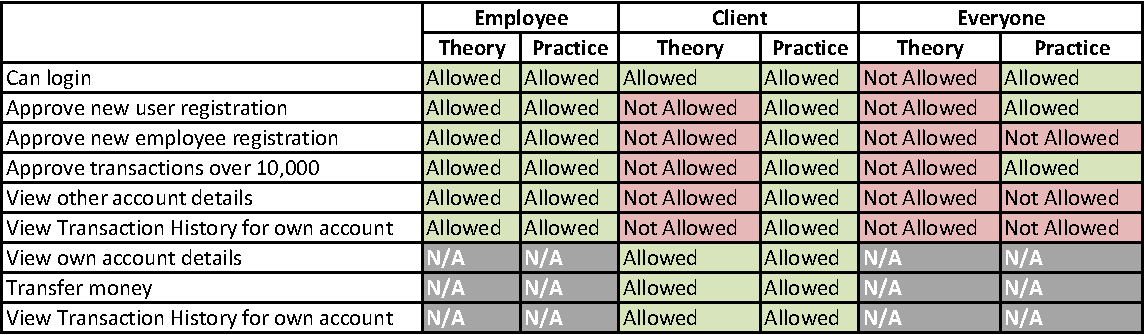
\includegraphics[width=\textwidth]{figures/RoleDefinitionsDoge}
	\caption{Role Definitions}
	\label{figure:RoleDefinitionsDoge}
\end{figure}


\vultable{\gnb}{%
	Clients, Employees and non-logged in users all act as expected, see \ref{figure:RoleDefinitionsGNB}
}{%
	This was verified through basic function testing and security testing tools (ZAP).
}{%
	N/A since no vulnerability was found.
}{%
	N/A 
}{%
\cvssBaseScorePretty{N}{L}{N}{N}{U}{L}{L}{L} %FIXME: This are mock values
}

\begin{figure}[h!tbp]
	\centering
	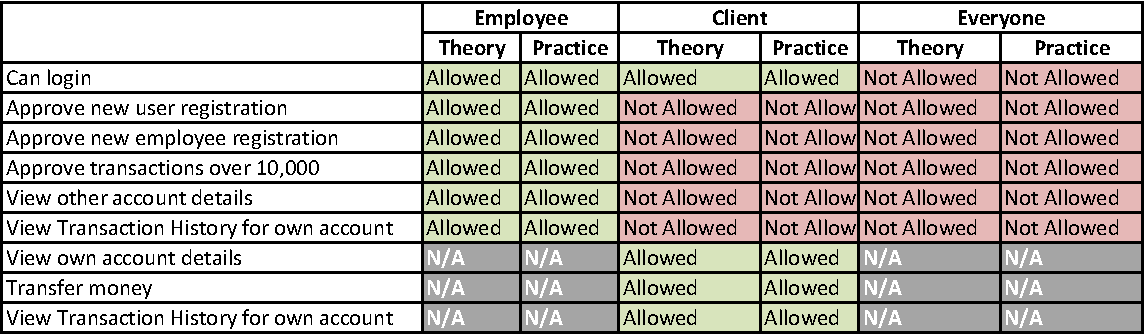
\includegraphics[width=\textwidth]{figures/RoleDefinitionsGNB}
	\caption{Role Definitions}
	\label{figure:RoleDefinitionsGNB}
\end{figure}


\vulntitle{OTG-IDENT-002}{Test User Registration Process}
\vultable{\doge}{%
	The registration process is set up for anyone to register, the process then awaits human interaction for the approval stage, this will serve an extra step of verification.

	Identities are not verified nor checked at this stage due to application limitations, email format verification is missing from the form.
}{%
	The email verification test was discovered through trail and error while registering.
}{%
	likely, due to intentional or unintentional mistyping.
}{%
	No serious impact as TAN codes are not sent to the email. 
}{%
\cvssBaseScorePretty{N}{L}{N}{N}{U}{L}{L}{L} %FIXME: This are mock values
}

\vultable{\gnb}{%
	The registration process is set up for anyone to register, the process then awaits human interaction for the approval stage, this will serve an extra step of verification.
	
	Identities are not verified nor checked at this stage due to application limitations.
}{%
	Trail and error.
}{%
	N/A since no vulnerability was found.
}{%
	N/A since no vulnerability was found. 
}{%
\cvssBaseScorePretty{N}{L}{N}{N}{U}{L}{L}{L} %FIXME: This are mock values
}

\vulntitle{OTG-IDENT-003}{Test Account Provisioning Process}
\vultable{\doge}{%
	The registration process is set up for anyone to register, the process then awaits human interaction for the approval stage, this will serve an extra step of verification.
	
	Identities are not verified nor checked at this stage due to application limitations, email format verification is missing from the form.
}{%
The email verification test was discovered through trail and error while registering.
}{%
likely, due to intentional or unintentional mistyping.
}{%
No serious impact as TAN codes are not sent to the email. 
}{%
\cvssBaseScorePretty{N}{L}{N}{N}{U}{L}{L}{L} %FIXME: This are mock values
}

\vultable{\gnb}{%
	The registration process is set up for anyone to register, the process then awaits human interaction for the approval stage, this will serve an extra step of verification.
	
	Identities are not verified nor checked at this stage due to application limitations, email format verification is missing from the form.
}{%
The email verification test was discovered through trail and error while registering.
}{%
likely, due to intentional or unintentional mistyping.
}{%
No serious impact as TAN codes are not sent to the email. 
}{%
\cvssBaseScorePretty{N}{L}{N}{N}{U}{L}{L}{L} %FIXME: This are mock values
}

\vulntitle{OTG-IDENT-004}{Testing for Account Enumeration and Guessable User Account}
\vulntitle{OTG-IDENT-005}{Testing for Weak or unenforced username policy}

\newpage
\section{Authentication Testing}	
\vulntitle{OTG-AUTHN-001}{Testing for Credentials Transported over an Encrypted Channel}
\vulntitle{OTG-AUTHN-002}{Testing for default credentials}
\vulntitle{OTG-AUTHN-003}{Testing for Weak lock out mechanism}
\vulntitle{OTG-AUTHN-004}{Testing for bypassing authentication schema}
\vulntitle{OTG-AUTHN-005}{Test remember password functionality}
\vulntitle{OTG-AUTHN-006}{Testing for Browser cache weakness}
\vulntitle{OTG-AUTHN-007}{Testing for Weak password policy}
\vulntitle{OTG-AUTHN-008}{Testing for Weak security question/answer}
\vulntitle{OTG-AUTHN-009}{Testing for weak password change or reset functionalities}
\vulntitle{OTG-AUTHN-010}{Testing for Weaker authentication in alternative channel}

\newpage
\section{Authorization Testing}
\vulntitle{OTG-AUTHZ-001}{Testing Directory traversal/file include}
\vulntitle{OTG-AUTHZ-002}{Testing for bypassing authorization schema}
\vulntitle{OTG-AUTHZ-003}{Testing for Privilege Escalation}
\vulntitle{OTG-AUTHZ-004}{Testing for Insecure Direct Object References}

\newpage
\section{Session Management Testing}
%SESSION 001
\vulntitle{OTG-SESS-001}{Testing for Bypassing Session Management Schema}
\vultable{\doge}{%
	When accessing the application, a randomly generated PHPSESSID session cookie is set. The cookie doesn't have an expiration date nor is it tagged as secure. Apparently the session cookie is already set before logging into the application. This cookie is simply replaced by a new one once the user logs out of the application. No other cookies are set. Also if the cookie is tampered with, the server automatically generates a new cookie, containing a new session ID.
}{%
	The PHPSESSID cookie has been discovered while intercepting HTTP requests/responses using Burp. The same cookie details were later on confirmed using the Cookies plugin for browser.
}{%
	\na
}{%
	Since the only used cookie only contains the session ID, even though it is easy to change the value of the cookie, no other session values are exposed to the user. It is still possible to hijack another session by changing the entire value of the cookie with the one associated to another user (see Session 004).
}{%
\na
}
\vultable{\gnb}{%
	The same observations made for the DogeBank application apply.
}{%
	The PHPSESSID cookie was analyzed using the Cookies plugin for browser.
}{%
	\na
}{%
	The same implications mentioned for the DogeBank application apply.
}{%
\na
}
%SESSION 002
\vulntitle{OTG-SESS-002}{Testing for Cookies attributes}
\vultable{\doge}{%
	observation text
}{%
discovery text
}{%
likelihood text
}{%
implication text
}{%
\cvssBaseScorePretty{N}{L}{N}{N}{U}{L}{L}{L} %FIXME: This are mock values
}
\vultable{\gnb}{%
	observation text
}{%
discovery text
}{%
likelihood text
}{%
implication text
}{%
\cvssBaseScorePretty{N}{L}{N}{N}{C}{L}{L}{L} %FIXME: This are mock values
}
%SESSION 003
\vulntitle{OTG-SESS-003}{Testing for Session Fixation}
%SESSION 004
\vulntitle{OTG-SESS-004}{Testing for Exposed Session Variables}
%SESSION 005
\vulntitle{OTG-SESS-005}{Testing for Cross Site Request Forgery}
%SESSION 006
\vulntitle{OTG-SESS-006}{Testing for logout functionality}
%SESSION 007
\vulntitle{OTG-SESS-007}{Test Session Timeout}
%SESSION 008
\vulntitle{OTG-SESS-008}{Testing for Session puzzling}

\newpage
\section{Data Validation Testing}
\vulntitle{OTG-INPVAL-001}{Testing for Reflected Cross Site Scripting}
\vulntitle{OTG-INPVAL-002}{Testing for Stored Cross Site Scripting}
\vulntitle{OTG-INPVAL-003}{Testing for HTTP Verb Tampering}
\vulntitle{OTG-INPVAL-004}{Testing for HTTP Parameter pollution}
\vulntitle{OTG-INPVAL-005}{Testing for SQL Injection}
\vulntitle{OTG-INPVAL-006}{Testing for LDAP Injection}
\vulntitle{OTG-INPVAL-007}{Testing for ORM Injection}
\vulntitle{OTG-INPVAL-008}{Testing for XML Injection}
\vulntitle{OTG-INPVAL-009}{Testing for SSI Injection}
\vulntitle{OTG-INPVAL-010}{Testing for XPath Injection}
\vulntitle{OTG-INPVAL-011}{IMAP/SMTP Injection}
\vulntitle{OTG-INPVAL-012}{Testing for Code Injection}
Testing for Local File Inclusion\\
Testing for Remote File Inclusion\\
\vulntitle{OTG-INPVAL-013}{Testing for Command Injection}
\vulntitle{OTG-INPVAL-014}{Testing for Buffer overflow}
Testing for Heap overflow\\
Testing for Stack overflow\\
Testing for Format string\\
\vulntitle{OTG-INPVAL-015}{Testing for incubated vulnerabilities}
\vulntitle{OTG-INPVAL-016}{Testing for HTTP Splitting/Smuggling}

\newpage
\section{Error Handling}
\vulntitle{OTG-ERR-001}{Analysis of Error Codes}
\vulntitle{OTG-ERR-002}{Analysis of Stack Traces}

\newpage
\section{Cryptography}
\vulntitle{OTG-CRYPST-001}{Testing for Weak SSL/TSL Ciphers, Insufficient Transport Layer Protection}
\vulntitle{OTG-CRYPST-002}{Testing for Padding Oracle}
\vulntitle{OTG-CRYPST-003}{Testing for Sensitive information sent via unencrypted channels}

\newpage
\section{Business Logic Testing}
\vulntitle{OTG-BUSLOGIC-001}{Test Business Logic Data Validation}
\vulntitle{OTG-BUSLOGIC-002}{Test Ability to Forge Requests}
\vulntitle{OTG-BUSLOGIC-003}{Test Integrity Checks}
\vulntitle{OTG-BUSLOGIC-004}{Test for Process Timing}
\vulntitle{OTG-BUSLOGIC-005}{Test Number of Times a Function Can be Used Limits}
\vulntitle{OTG-BUSLOGIC-006}{Testing for the Circumvention of Work Flows}
\vulntitle{OTG-BUSLOGIC-007}{Test Defenses Against Application Mis-use}
\vulntitle{OTG-BUSLOGIC-008}{Test Upload of Unexpected File Types}
\vulntitle{OTG-BUSLOGIC-009}{Test Upload of Malicious Files}

\newpage
\section{Client Side Testing}
This section was prioritized as low, therefore the client side was not tested in depth. Furthermore, as stated in the OWASP testing guide, black box testing of the client side is usually not performed, since access to the source code is always available, as it needs to be sent to the client to be executed. Nevertheless, some potential vulnerabilities were found and briefly analyzed.
\vulntitle{OTG-CLIENT-001}{Testing for DOM based Cross Site Scripting}
\vulntitle{OTG-CLIENT-002}{Testing for JavaScript Execution}
\vulntitle{OTG-CLIENT-003}{Testing for HTML Injection}
\vulntitle{OTG-CLIENT-004}{Testing for Client Side URL Redirect}
\vulntitle{OTG-CLIENT-005}{Testing for CSS Injection}
\vulntitle{OTG-CLIENT-006}{Testing for Client Side Resource Manipulation}
\vulntitle{OTG-CLIENT-007}{Test Cross Origin Resource Sharing}
\vulntitle{OTG-CLIENT-008}{Testing for Cross Site Flashing}
\vulntitle{OTG-CLIENT-009}{Testing for Clickjacking}
\vulntitle{OTG-CLIENT-010}{Testing WebSockets}
\vulntitle{OTG-CLIENT-011}{Test Web Messaging}
\vulntitle{OTG-CLIENT-012}{Test Local Storage}
